\section{BriskSeed Design}
\label{sec:briskseed-design}

This section presents the full BriskSeed design for dynamic ANNS under continuous updates.
Section 3.1 introduces the design overview.
Section 3.2 describes the overall pipeline of BriskSeed.
Section 3.3 gives complexity, robustness, and challenge-wise implications.

\subsection{Design Overview}


Motivated by the observations and challenges in Section~2, we design \textbf{BriskSeed} as a three-layer online framework for accelerating dynamic ANNS. 
BriskSeed is built on a simple principle: historical search outcomes, referred to as \emph{seeds}, should be reused only when they can be represented compactly, activated selectively, and trusted safely under continuous updates. 
To this end, BriskSeed combines three layers that map directly to the three challenges in Section~2: Seed Storage Layer, Seed-Guided Search Layer, and Reliability Control Layer, as shown in Figure~\ref{fig:briskseed-design-overview}.

\noindent\textbf{(1) Seed Storage Layer (addresses Challenge 1).}
This layer determines how historical outcomes are represented, retained, and refreshed under bounded memory. 
To exploit the high top-$k$ overlap across nearby rounds, BriskSeed organizes reusable history in a two-tier seed storage: a hot-exact tier for highly recurring outcomes and a semantic-shared tier for compact long-tail coverage. 
Each seed stores historical top-$k$ IDs together with lightweight metadata needed for retrieval and maintenance. 
In this way, past outcomes are encoded as reusable guidance rather than final answers, while retention and eviction remain explicitly budgeted.

\noindent\textbf{(2) Seed-Guided Search Layer (addresses Challenge 2).}
This layer determines how stored outcomes guide query-time search. 
For each query, BriskSeed first retrieves seeds through exact lookup or bounded semantic probing, and then converts the selected seed into provisional candidates through bounded expansion. 
The guidance strategy is tier-aware: hot-exact seeds use one-hop neighbor expansion by default, while semantic-shared seeds use guarded multi-hop expansion only when one-hop evidence
is insufficient.
This design enables efficient reuse under skewed workloads while preventing uncontrolled search overhead.

\noindent\textbf{(3) Reliability Control Layer (addresses Challenge 3).}
This layer ensures that reuse improves end-to-end efficiency without degrading recall. 
Recovered candidates are checked by a lightweight query-level acceptance policy, where acceptance requires both strong local candidate quality and consistency with the seed's historical neighborhood. 
If either signal is weak, BriskSeed immediately falls back to the native search path. 
This explicit reliability gate ensures that acceleration remains beneficial while bounding recall risk.

These three layers are co-designed rather than independent. 
The seed storage layer determines what is reusable, the seed-guided search layer determines how reuse enters search, and the reliability control layer determines when recovered candidates are trustworthy enough to be accepted. 
Together, they form a bounded online reuse framework that aligns directly with the three design challenges and remains robust under continuous updates.



\begin{figure}[t]
\centering
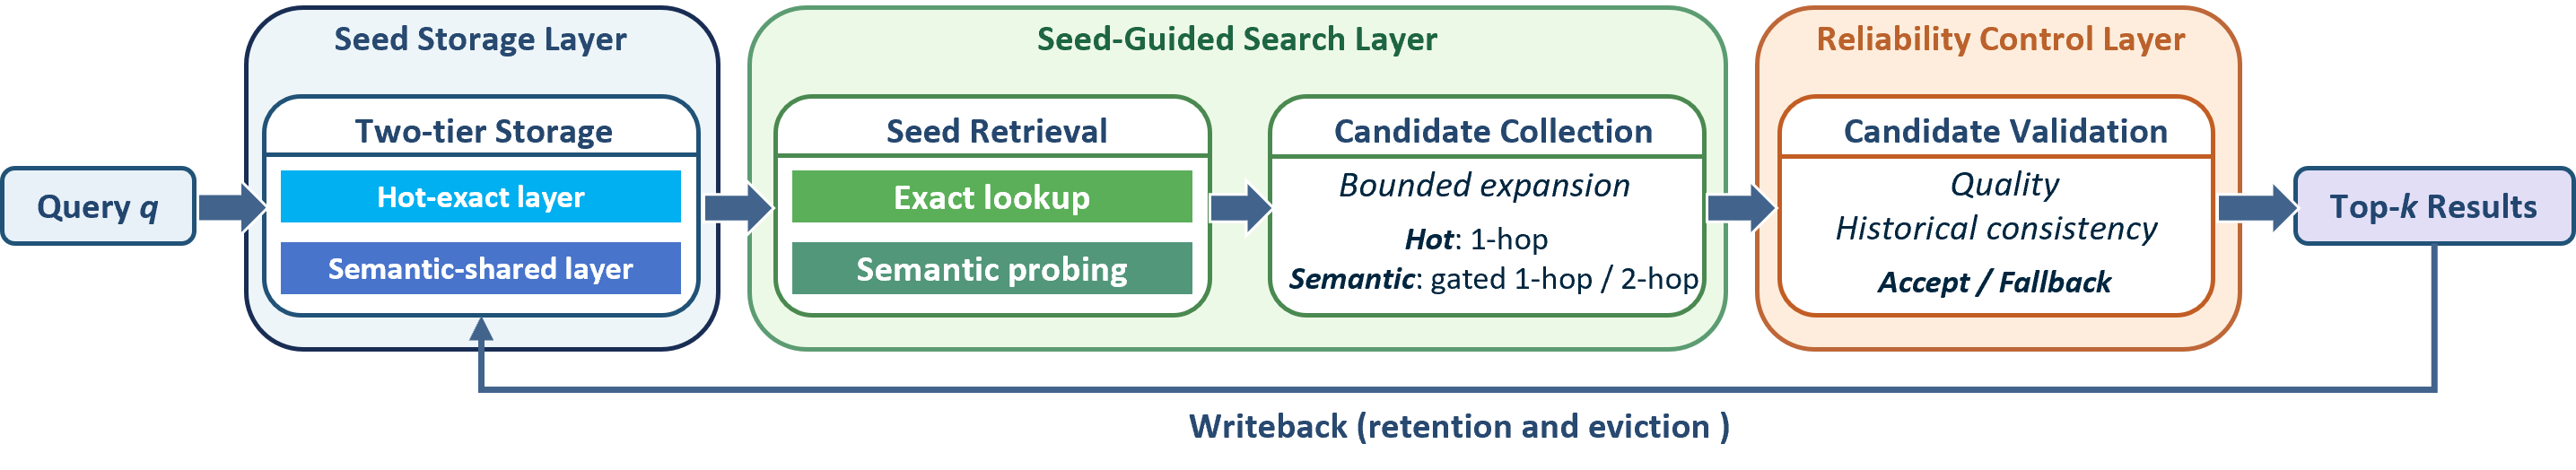
\includegraphics[width=\columnwidth]{figures/figure3.png}
\caption{BriskSeed design overview.}
\label{fig:briskseed-design-overview}
\end{figure}




\subsection{Unified Online Reuse Pipeline}
In this subsection, we detail the modules of BriskSeed and their interactions in the unified online reuse pipeline. Important symbols are summarized in Table~\ref{tab:pipeline-symbols}.

\subsubsection{Seed representation and storage}

\paragraph{Seed representation.}
We first define the representation of a seed, and then describe how such seeds are organized in the storage.

Each seed is stored as
\begin{equation}
r=\langle \mathbf{z}, n_b, \beta, \rho \rangle,
\end{equation}
where $\mathbf{z}\in\mathbb{N}^k$ is the historical top-$k$ result IDs used as reuse anchors, $n_b$ is the seed birth time (when the seed was created), $\beta$ identifies the source query ID (which query generated this seed), and $\rho$ records the successful reuse count. The anchor set $\mathbf{z}$ serves as the starting points for subsequent reuse, 
while the remaining metadata summarize freshness, origin, and past effectiveness, respectively. 
Among them, $\beta$ and $\rho$ are used directly during seed retrieval, whereas $n_b$ is primarily used later for seed retention and eviction.

\paragraph{Two-tier seed storage.}
Given the seed representation above, BriskSeed organizes reusable seeds in a two-tier storage, consisting of a \textit{hot-exact} layer and a \textit{semantic-shared} layer, to balance reuse 
quality and storage cost. The hot-exact layer is organized as a bounded key-value store with capacity $H$, where each query ID maps to a unique seed, enabling constant-time 
lookup for highly recurring queries. In contrast, the semantic-shared layer is organized as an array of $S$ slots, each storing up to $m$ seeds, to provide bounded long-tail 
coverage. To route queries to semantic slots, BriskSeed derives a lightweight query signature $\phi(q)$ from the query vector using a coarse projection (e.g., random 
projection or product quantization) that preserves approximate semantic information while remaining inexpensive to compute. The signature is used only for seed routing and does 
not participate in the ANN search.

A single-layer design is practically insufficient. 
Storing one seed per query in dedicated exact slots yields highly aligned retrieval but incurs prohibitive memory growth under dynamic workloads. 
Conversely, if all seeds are placed in a fully shared semantic array where queries are routed to shared slots via signatures, memory usage would be reduced but may return 
loosely matched seeds that require deeper multi-hop expansion, offsetting the benefit of reuse. 
The two-tier design balances these extremes: the hot-exact layer serves recurrent, high-value patterns, while the semantic-shared layer provides compact coverage for remaining massive yet low-utility historical outcomes.


\begin{table}[t]
	\caption{Symbols used in BriskSeed design.}
	\label{tab:pipeline-symbols}
	\centering
	%\footnotesize
	\setlength{\tabcolsep}{3pt}
	\begin{tabular}{p{2.35cm}p{5.75cm}}
		\toprule
		Symbol & Description \\
		\midrule
		\multicolumn{2}{l}{\textit{Storage and Retrieval}} \\
		$q$ & Incoming query. \\
		$\phi(q)$ & Query signature for semantic routing. \\
		$g(q),\ s(q),\ \mathcal{N}(q)$ & Hot-key, semantic slot key, and probed semantic neighborhood. \\
		$S,\ m,\ P,\ H$ & Semantic slot count, per-slot seed upper limit, probing-width limit, and hot-layer capacity. \\
		$r=\langle\mathbf{z},n_b,\beta,\rho\rangle$ & Record of a seed: historical top-$k$ IDs, birth time, source query ID, and accepted-reuse count. \\
		$u(r)$ & Priority score of seed $r$ for seed ranking. \\
		\midrule
		\multicolumn{2}{l}{\textit{Validation}} \\
		$d(\cdot,\cdot)$ & Backend distance metric. \\
		$\hat{\mathbf{z}}$ & Recovered provisional top-$k$ set. \\
		$\mathrm{qual}(q),\ \mathrm{cons}(q)$ & Candidate quality and overlap-consistency signals for acceptance. \\
		\midrule
		\multicolumn{2}{l}{\textit{Writeback and Maintenance}} \\
		$\mathrm{keep}(r)$ & Keep score of seed $r$ for eviction. \\
		$n,\ \mathrm{age}_n(r)$ & Processed-query counter and on-demand seed age $\mathrm{age}_n(r)=n-n_b$. \\
		\bottomrule
	\end{tabular}
\end{table}
\iffalse
Given a query $q$, BriskSeed computes two indexing keys:
\begin{equation}
g(q) = \mathrm{id}(q), \qquad
s(q) = \operatorname{hash}(\phi(q)) \bmod S.
\end{equation}
The key $g(q)$ is used to check whether an exact seed for this query already exists in the hot-exact layer, enabling immediate warm-start reuse when available. 
The key $s(q)$ maps the query to a semantic slot for shared reuse. 
To increase retrieval robustness, BriskSeed probes a small neighborhood of nearby slots
\begin{equation}
\mathcal{N}(q) = \{s_1(q),\ldots,s_P(q)\}, \qquad P \ll S ,
\end{equation}
where $s_1(q)=s(q)$ and the remaining slots are obtained through lightweight offset probing. 
This bounded probing increases the likelihood of finding a useful seed while keeping lookup overhead low.
\fi

\subsubsection{Seed-guided search}
\paragraph{Seed retrieval.}

At query time, BriskSeed first attempts to retrieve reusable seeds from the two-tier seed storage. 

Given a query $q$, it computes two indexing keys:
\begin{equation}
g(q) = \mathrm{id}(q), \qquad
s(q) = \operatorname{hash}(\phi(q)) \bmod S .
\end{equation}
The key $g(q)$ is used for exact lookup in the hot layer, while the key $s(q)$ routes the query to a semantic slot in the shared layer. 
%{\color{blue}At this stage, control-layer budget $P_t$ determines the semantic probing width, so retrieval cost is explicitly bounded by $O(P_t\cdot m)$ candidate inspections.}
If a matching entry is indeed found in the hot layer, BriskSeed directly reuses the associated seed. 
Because the hot-layer seed is keyed by the same query ID, it is tightly aligned with the current query. 

Otherwise, BriskSeed probes a small neighborhood of semantic slots, because seeds in the primary slot alone may be insufficiently aligned with the current query.
\begin{equation}
\mathcal{N}(q)=\{s(q),s(q)+1, \ldots,s(q)+P-1\}, \qquad P \ll S.
\end{equation}
i.e., the primary slot $s(q)$ together with its $P-1$ consecutive offset probes.
Here, $P$ is a manually controlled upper bound on semantic probing width, so probing inspects at most $P$ slots with up to $m$ seeds each, yielding a bounded retrieval cost of $O(Pm)$.
All candidate seeds in the union of probed slots are then assigned a lightweight priority score:
\begin{equation}
u(r)=\lambda\,\mathrm{sim}(\phi(q),\beta)
+(1-\lambda)\,\rho.
\end{equation}
Here, $\mathrm{sim}(\phi(q),\beta)$ measures the match between the current query signature and the seed's source signature and $\rho$ records 
how many times the seed has previously led to successful reuse.
Based on these scores, BriskSeed selects the top-ranked seed as the warm-start anchor.



\paragraph{Candidate Collection.}


Given a selected seed, BriskSeed performs bounded candidate recovery on the graph index using the seed's result nodes as starting points. 
For hot-exact seeds, the retrieved seed is tightly aligned with the query, so BriskSeed adopts one-hop neighbor expansion by default. 
In this process, BriskSeed retains the nodes recorded in the seed and expands one hop from them to collect their immediate neighbors, and the union of both forms the candidate set.
This preserves the historical top-$k$ results while incorporating a local correction to account for recent batch updates.
As we show later in the evaluation, this low-overhead one-hop design is sufficient to recover strong candidates in most cases.

For semantic-shared seeds, one-hop expansion may not always recover sufficiently strong candidates because the retrieved seed is only approximately aligned with the query. 
BriskSeed therefore first performs one-hop expansion and examines the best candidate obtained. 
If the best one-hop candidate is still not close enough to the query judged by a distance gate, recovery continues to a two-hop; otherwise, it stops after one-hop. 
Recovery is capped at two hops, since deeper exploration leads to rapid frontier growth and empirically yields diminishing returns.

Given the recovered candidate set, BriskSeed ranks candidates under the backend distance metric and truncates them to form a provisional top-$k$ set, denoted by $\hat{\mathbf{z}}$. 
When neither memory tier yields a reusable seed, the system falls back to the baseline graph-based ANN search to produce the final top-$k$ results. 
Thus, seed reuse is opportunistic rather than mandatory.



\subsubsection{Candidate Validation}

The bounded recovery stage produces only a provisional top-$k$ result $\hat{\mathbf{z}}$, which BriskSeed does not accept blindly. 
Instead, it applies a lightweight query-level acceptance-and-fallback policy based on two signals: candidate quality and historical consistency.

For candidate quality, let $c_1$ and $c_2$ denote the best and second-best candidates in the recovered set under the backend distance metric $d(\cdot,\cdot)$. 
BriskSeed computes the normalized winner-quality signal
\begin{equation}
\mathrm{qual}(q)=\frac{d(q,c_2)-d(q,c_1)}{d(q,c_1)+\epsilon},
\end{equation}
where $\epsilon>0$ is a small constant for numerical stability. 
This signal favors provisional results in which the best recovered candidate is not only close to the query, but also clearly separated from its closest competitor. 
A small value of $\mathrm{qual}(q)$ indicates that the current recovered set does not yet provide a sufficiently reliable winner.

For overlap consistency, BriskSeed compares the top-$k$ results of the recovered candidate set, denoted by $\hat{\mathbf{z}}$, with the historical top-$k$ set $\mathbf{z}$ stored in the seed, and computes
\begin{equation}
\mathrm{cons}(q)=\frac{|\hat{\mathbf{z}}\cap \mathbf{z}|}{k}.
\end{equation}
This signal measures the overlap between the provisional top-$k$ recovered for the current query and what the seed previously contributed. 
If overlap is low, the local structure has likely drifted, so reuse is unlikely to help and should be rejected.

The recovered result is accepted only when both signals satisfy their acceptance thresholds; otherwise, BriskSeed falls back to the baseline graph-based ANN search.
This conjunction avoids two failure modes: high $\mathrm{qual}(q)$ but low $\mathrm{cons}(q)$, and high $\mathrm{cons}(q)$ but low $\mathrm{qual}(q)$.
Therefore, BriskSeed keeps only provisional results with both strong local candidate quality and sufficient overlap with the seed's stored top-$k$ results.



\subsubsection{Writeback mechanism and seed update}

After each query finishes, BriskSeed writes the final top-$k$ results back to update seed statistics and memory contents. 
This writeback is performed for every query, regardless of whether the result comes from the hot-exact path, the semantic-shared path, or the baseline fallback. 




If the query already has an entry in the hot-exact layer, BriskSeed directly updates the corresponding key-value record under the same query ID. 
Otherwise, the resulting seed is inserted into the semantic-shared layer according to its semantic slot. 
If the target semantic slot is full, eviction is governed by the keep score
\begin{equation}
\mathrm{keep}(r)=\xi\,\rho-(1-\xi)\,\mathrm{age}_n(r), \quad \mathrm{age}_n(r)=n-n_b.
\end{equation}
where $n$ is the cumulative number of processed queries so far.
Seeds with low keep score are evicted from the corresponding semantic slot to maintain it upper threshold.
Over time, this writeback process also adjusts seed placement across the two tiers. 
Promotion and demotion are decided when a seed is used, based on its successful reuse count $\rho$ and age $\mathrm{age}_n(r)$. Semantic seeds with high reuse utility and recent birth are promoted to the hot-exact layer, while hot seeds with low reuse utility or old age are moved back to the semantic-shared layer.
Overall, this policy keeps high-value seeds in memory while gradually removing stale or ineffective ones.

\subsection{Cost Model and Decision Model}

To make BriskSeed practical under fixed memory and latency budgets, we use a lightweight online decision model to set the hot/semantic split and probing parameters.

\paragraph{Budget split between hot and semantic layers.}
Let $B$ be the total seed budget (in number of seed records). We split it as
\begin{equation}
H=\lfloor \alpha B \rfloor, \qquad Sm = B-H,
\end{equation}
where $\alpha\in(0,1)$ is the hot-layer ratio, $H$ is hot-layer capacity, and $S,m$ are semantic slot count and per-slot cap.
Thus, $\alpha$ directly controls the trade-off: larger $\alpha$ favors exact reuse for highly recurring queries, while smaller $\alpha$ favors broader long-tail coverage.

\paragraph{Expected query cost model.}
For one query, define: $p_h$ as hot-hit rate, $p_s$ as semantic-hit rate when hot misses, and $p_a$ as acceptance rate after seed-guided recovery.
Let $C_h$ be hot-hit path cost, $C_s$ semantic-reuse path cost (including probing/recovery/validation), and $C_b$ baseline native-search cost.
Then the expected cost is
\begin{equation}
\mathbb{E}[C] = p_h C_h + (1-p_h)\Big(p_s\big(p_a C_s + (1-p_a)C_b\big) + (1-p_s)C_b\Big).
\end{equation}
This form makes the decision objective explicit: maximize $p_h$ and $p_s p_a$ while keeping $C_s$ bounded by probing and recovery budgets.

\paragraph{Decision objective and constraints.}
We choose $(\alpha, P, m)$ to minimize $\mathbb{E}[C]$ under two constraints:
\begin{equation}
\mathrm{Recall} \ge \tau \cdot \mathrm{Recall}_{\mathrm{baseline}},
\end{equation}
\begin{equation}
Pm \le K_{\max},
\end{equation}
where $\tau$ is the recall ratio target and $K_{\max}$ is a fixed retrieval budget.
The first constraint prevents over-aggressive reuse; the second keeps semantic-stage overhead bounded.

\paragraph{Online parameter setting in practice.}
We estimate $p_h,p_s,p_a,C_h,C_s,C_b$ from moving averages over recent rounds and update parameters every $T$ rounds using a small candidate set.
Specifically, we evaluate candidate $\alpha$ values (e.g., $\{0.2,0.3,0.4,0.5\}$) and candidate $(P,m)$ pairs satisfying $Pm\le K_{\max}$, then pick the lowest-cost feasible configuration.
This yields a stable and low-overhead controller: hot/semantic partition adapts to workload skew, while probing depth and per-slot fan-in remain bounded.

\subsection{Time Complexity and Feasibility Analysis}
\label{subsec:briskseed-complexity}

We next analyze whether BriskSeed can reduce query-time cost in principle, using HNSW-style graph search as the reference baseline.
Let $C_{\text{hnsw}}$ denote the average distance-computation cost of one baseline query under a fixed recall target.

\paragraph{Per-query overhead of BriskSeed.}
For one query, BriskSeed adds four lightweight stages before deciding reuse or fallback.
\textit{(i) Seed lookup.} Hot-layer lookup is constant-time, while semantic probing inspects at most $P$ slots and at most $m$ seeds per slot, yielding $O(Pm)$ seed inspections.
\textit{(ii) Seed scoring and selection.} Ranking the inspected seeds is also bounded by $O(Pm)$.
\textit{(iii) Bounded candidate recovery.} Starting from top-$k$ anchors, one-hop or guarded two-hop expansion is capped by design, so its work is bounded by a small constant factor times $k$ and local graph degree, rather than a full best-first traversal.
\textit{(iv) Validation and writeback.} Computing $\mathrm{qual}(q)$, $\mathrm{cons}(q)$, and updating one seed record are linear in the recovered candidate size and thus bounded by the same capped frontier.

Hence, when reuse is accepted, BriskSeed query cost is dominated by bounded probing plus bounded local expansion, i.e., a capped local procedure instead of global graph exploration.
Under fixed system budgets ($P$, $m$, and short-hop depth), this reuse path is $O(1)$ with respect to dataset size $N$.

\paragraph{Comparison to standard graph-based ANNS (HNSW).}
The original HNSW paper reports logarithmic complexity scaling with dataset size, while in practice per-query search cost is mainly controlled by the traversal budget needed for a target recall (typically reflected by \\texttt{efSearch}).
In baseline HNSW, each query pays this traversal cost.
In BriskSeed, an accepted reuse replaces the full traversal with a bounded local procedure.
Let $C_{\text{reuse}}$ denote the full bounded cost of one reuse attempt (lookup, scoring, capped recovery, validation, and writeback), and let $p_{\text{acc}}$ denote the acceptance rate.
Then BriskSeed's expected query cost is upper-bounded by
\begin{equation}
\mathbb{E}[C_{\text{stream}}]
\le C_{\text{reuse}} + (1-p_{\text{acc}})\,C_{\text{hnsw}}.
\end{equation}
Therefore, a sufficient condition for latency improvement over native HNSW is
\begin{equation}
C_{\text{reuse}} < p_{\text{acc}}\,C_{\text{hnsw}}.
\end{equation}
This inequality directly explains when BriskSeed is faster: reuse itself must be cheaper than native traversal, and this advantage must occur often enough (high $p_{\text{acc}}$).
Since $C_{\text{reuse}}$ is capped by $P$, $m$, and short-hop recovery, the left-hand side remains bounded by design.
Consequently, as $N$ grows, BriskSeed preserves a bounded accepted-reuse cost while native HNSW search still grows approximately logarithmically; this creates an increasing asymptotic gap between one accepted reuse and one native search.

\paragraph{Feasibility under dynamic updates.}
Continuous updates mainly affect seed validity, not the complexity bound itself.
BriskSeed keeps complexity stable through two mechanisms: bounded probing/recovery prevents unbounded per-query growth, and acceptance gating prevents low-quality reuse from replacing baseline search.
As a result, dynamic drift lowers optimization gain primarily by reducing $p_{\text{acc}}$, while correctness is preserved by fallback and worst-case time remains comparable to baseline HNSW.

